%%%%%%%%%%%%%%%%%%%%%%%%%%%%%%%%%%%%%%%%%
% Beamer Presentation
% LaTeX Template
% Version 1.0 (10/11/12)
%
% This template has been downloaded from:
% http://www.LaTeXTemplates.com
%
% License:
% CC BY-NC-SA 3.0 (http://creativecommons.org/licenses/by-nc-sa/3.0/)
%
%%%%%%%%%%%%%%%%%%%%%%%%%%%%%%%%%%%%%%%%%

%----------------------------------------------------------------------------------------
%	PACKAGES AND THEMES
%----------------------------------------------------------------------------------------

\documentclass{beamer}

\mode<presentation> {

% The Beamer class comes with a number of default slide themes
% which change the colors and layouts of slides. Below this is a list
% of all the themes, uncomment each in turn to see what they look like.

%\usetheme{default}
%\usetheme{AnnArbor}
%\usetheme{Antibes}
%\usetheme{Bergen}
%\usetheme{Berkeley}
%\usetheme{Berlin} % fancy navigations anzeige
%\usetheme{Boadilla} %schön aufgeräumt und hell
%\usetheme{CambridgeUS} % anzeige des aktuellen section und subsection, recht schick
%\usetheme{Copenhagen}
%\usetheme{Darmstadt} %fancy navigations anzeige
%\usetheme{Dresden}
%\usetheme{Frankfurt}%fancy navigations anzeige, kleine auflistungspunkte
%\usetheme{Goettingen} %Navigationsleiste rechts, recht schick, default sonst
%\usetheme{Hannover}
%\usetheme{Ilmenau} % fancy navigations anzeige, mit anzeige der subsection
%\usetheme{JuanLesPins}% anzeige des aktuellen section und subsection
%\usetheme{Luebeck}
% %\usetheme{Madrid}
%\usetheme{Malmoe}
%\usetheme{Marburg}
\usetheme{Montpellier}% anzeige des aktuellen section und subsection, sehr hell
%\usetheme{PaloAlto}
%\usetheme{Pittsburgh}
%\usetheme{Rochester} %quadrate als punkte
%\usetheme{Singapore} % fancy navigations anzeige, hell
%\usetheme{Szeged}
%\usetheme{Warsaw}

% As well as themes, the Beamer class has a number of color themes
% for any slide theme. Uncomment each of these in turn to see how it
% changes the colors of your current slide theme.

%\usecolortheme{albatross}
%\usecolortheme{beaver}
%\usecolortheme{beetle}
%\usecolortheme{crane}
%\usecolortheme{dolphin}
%\usecolortheme{dove}
%\usecolortheme{fly}
%\usecolortheme{lily}
%\usecolortheme{orchid}
%\usecolortheme{rose}
%\usecolortheme{seagull}
%\usecolortheme{seahorse}
%\usecolortheme{whale}
%\usecolortheme{wolverine}

%\setbeamertemplate{footline} % To remove the footer line in all slides uncomment this line
%\setbeamertemplate{footline}[page number] % To replace the footer line in all slides with a simple slide count uncomment this line

\setbeamertemplate{navigation symbols}{} % To remove the navigation symbols from the bottom of all slides uncomment this line
}
\setbeamertemplate{footline}[frame number]
\setbeamerfont{page number in head/foot}{size=\scriptsize}

\usepackage{graphicx} % Allows including images
\usepackage{booktabs} % Allows the use of \toprule, \midrule and \bottomrule in tables
\usepackage{csvsimple}
\usepackage[position=b,singlelinecheck=off]{subfig}
\usepackage{caption}
\usepackage{float}
\usepackage{selinput}      % Halbautomatische Auswahl der Eingabecodierung
\SelectInputMappings{      % mit Hilfe ausgewählter Glyphen
  adieresis={ä},	   % siehe: http://partners.adobe.com/public/developer/en/opentype/glyphlist.txt
  germandbls={ß},
  Euro={€}
}

%----------------------------------------------------------------------------------------
%	TITLE PAGE
%----------------------------------------------------------------------------------------

\title[Predicting I/O-performance]{Predicting I/O-performance in HPC using Artificial Neural Networks} % The short title appears at the bottom of every slide, the full title is only on the title page

%\author{Jan Fabian Schmid} % Your name
\author[Jan Fabian Schmid]{Jan Fabian Schmid\\{\small Tutor: Dr. Julian Kunkel}}
\institute[UHH] % Your institution as it will appear on the bottom of every slide, may be shorthand to save space
{
University of Hamburg \\ % Your institution for the title page
\medskip
\textit{2schmid@informatik.uni-hamburg.de} % Your email address
}
\date{21.06.2016} % Date, can be changed to a custom date

\makeatletter
\newenvironment{withoutheadline}{
	\setbeamertemplate{headline}[default]
	\def\beamer@entrycode{\vspace*{-\headheight}}
}{}
\makeatother

\newcommand{\backupbegin}{
	\newcounter{finalframe}
	\setcounter{finalframe}{\value{framenumber}}
}
\newcommand{\backupend}{
	\setcounter{framenumber}{\value{finalframe}}
}

\begin{document}
\setbeamertemplate{caption}{\raggedright\insertcaption\par}
\setbeamerfont{caption}{size=\scriptsize}

\begin{withoutheadline}
	\begin{frame}[plain]
		\titlepage % Print the title page as the first slide
	\end{frame}
\end{withoutheadline}


%\section*{Übersicht}
%\begin{withoutheadline}
%	\begin{frame}
%		\frametitle{Übersicht} % Table of contents slide, comment this block out to remove it
%		\tableofcontents % Throughout your presentation, if you choose to use \section{} and \subsection{} commands, these will automatically be printed on this slide as an overview of your presentation
%	\end{frame}
%\end{withoutheadline}

%----------------------------------------------------------------------------------------
%	PRESENTATION SLIDES
%----------------------------------------------------------------------------------------

\section{Introduction}

\subsection{Goals and problems}
\begin{withoutheadline}
	\begin{frame}
		\frametitle{Introduction}
		\begin{itemize}
			\item Prediction of file access times to model storage systems
			\item Models can be used to develop supportive tools
			\item Analytical models are not feasible
			\item We used Artificial Neural Networks (ANNs) for prediction
		\end{itemize}
	\end{frame}
\end{withoutheadline}

\begin{withoutheadline}
	\begin{frame}
		\frametitle{Measurements}
		\begin{itemize}
			\item File access times were measured for different access patterns
			%\item We analyzed different access patterns
			\item \textbf{File accesses with equal parameter values have several typical access times}
			\item This is caused through varying processing (I/O-paths) in the storage system
			%this is therefore very important information for the predictions, but we cant directly measure them
			\item Error classes method to exploit knowledge about I/O-paths to analyze the importance for access time prediction
		\end{itemize}
		\begin{columns}
			\column{.5\textwidth}
			\begin{figure}
				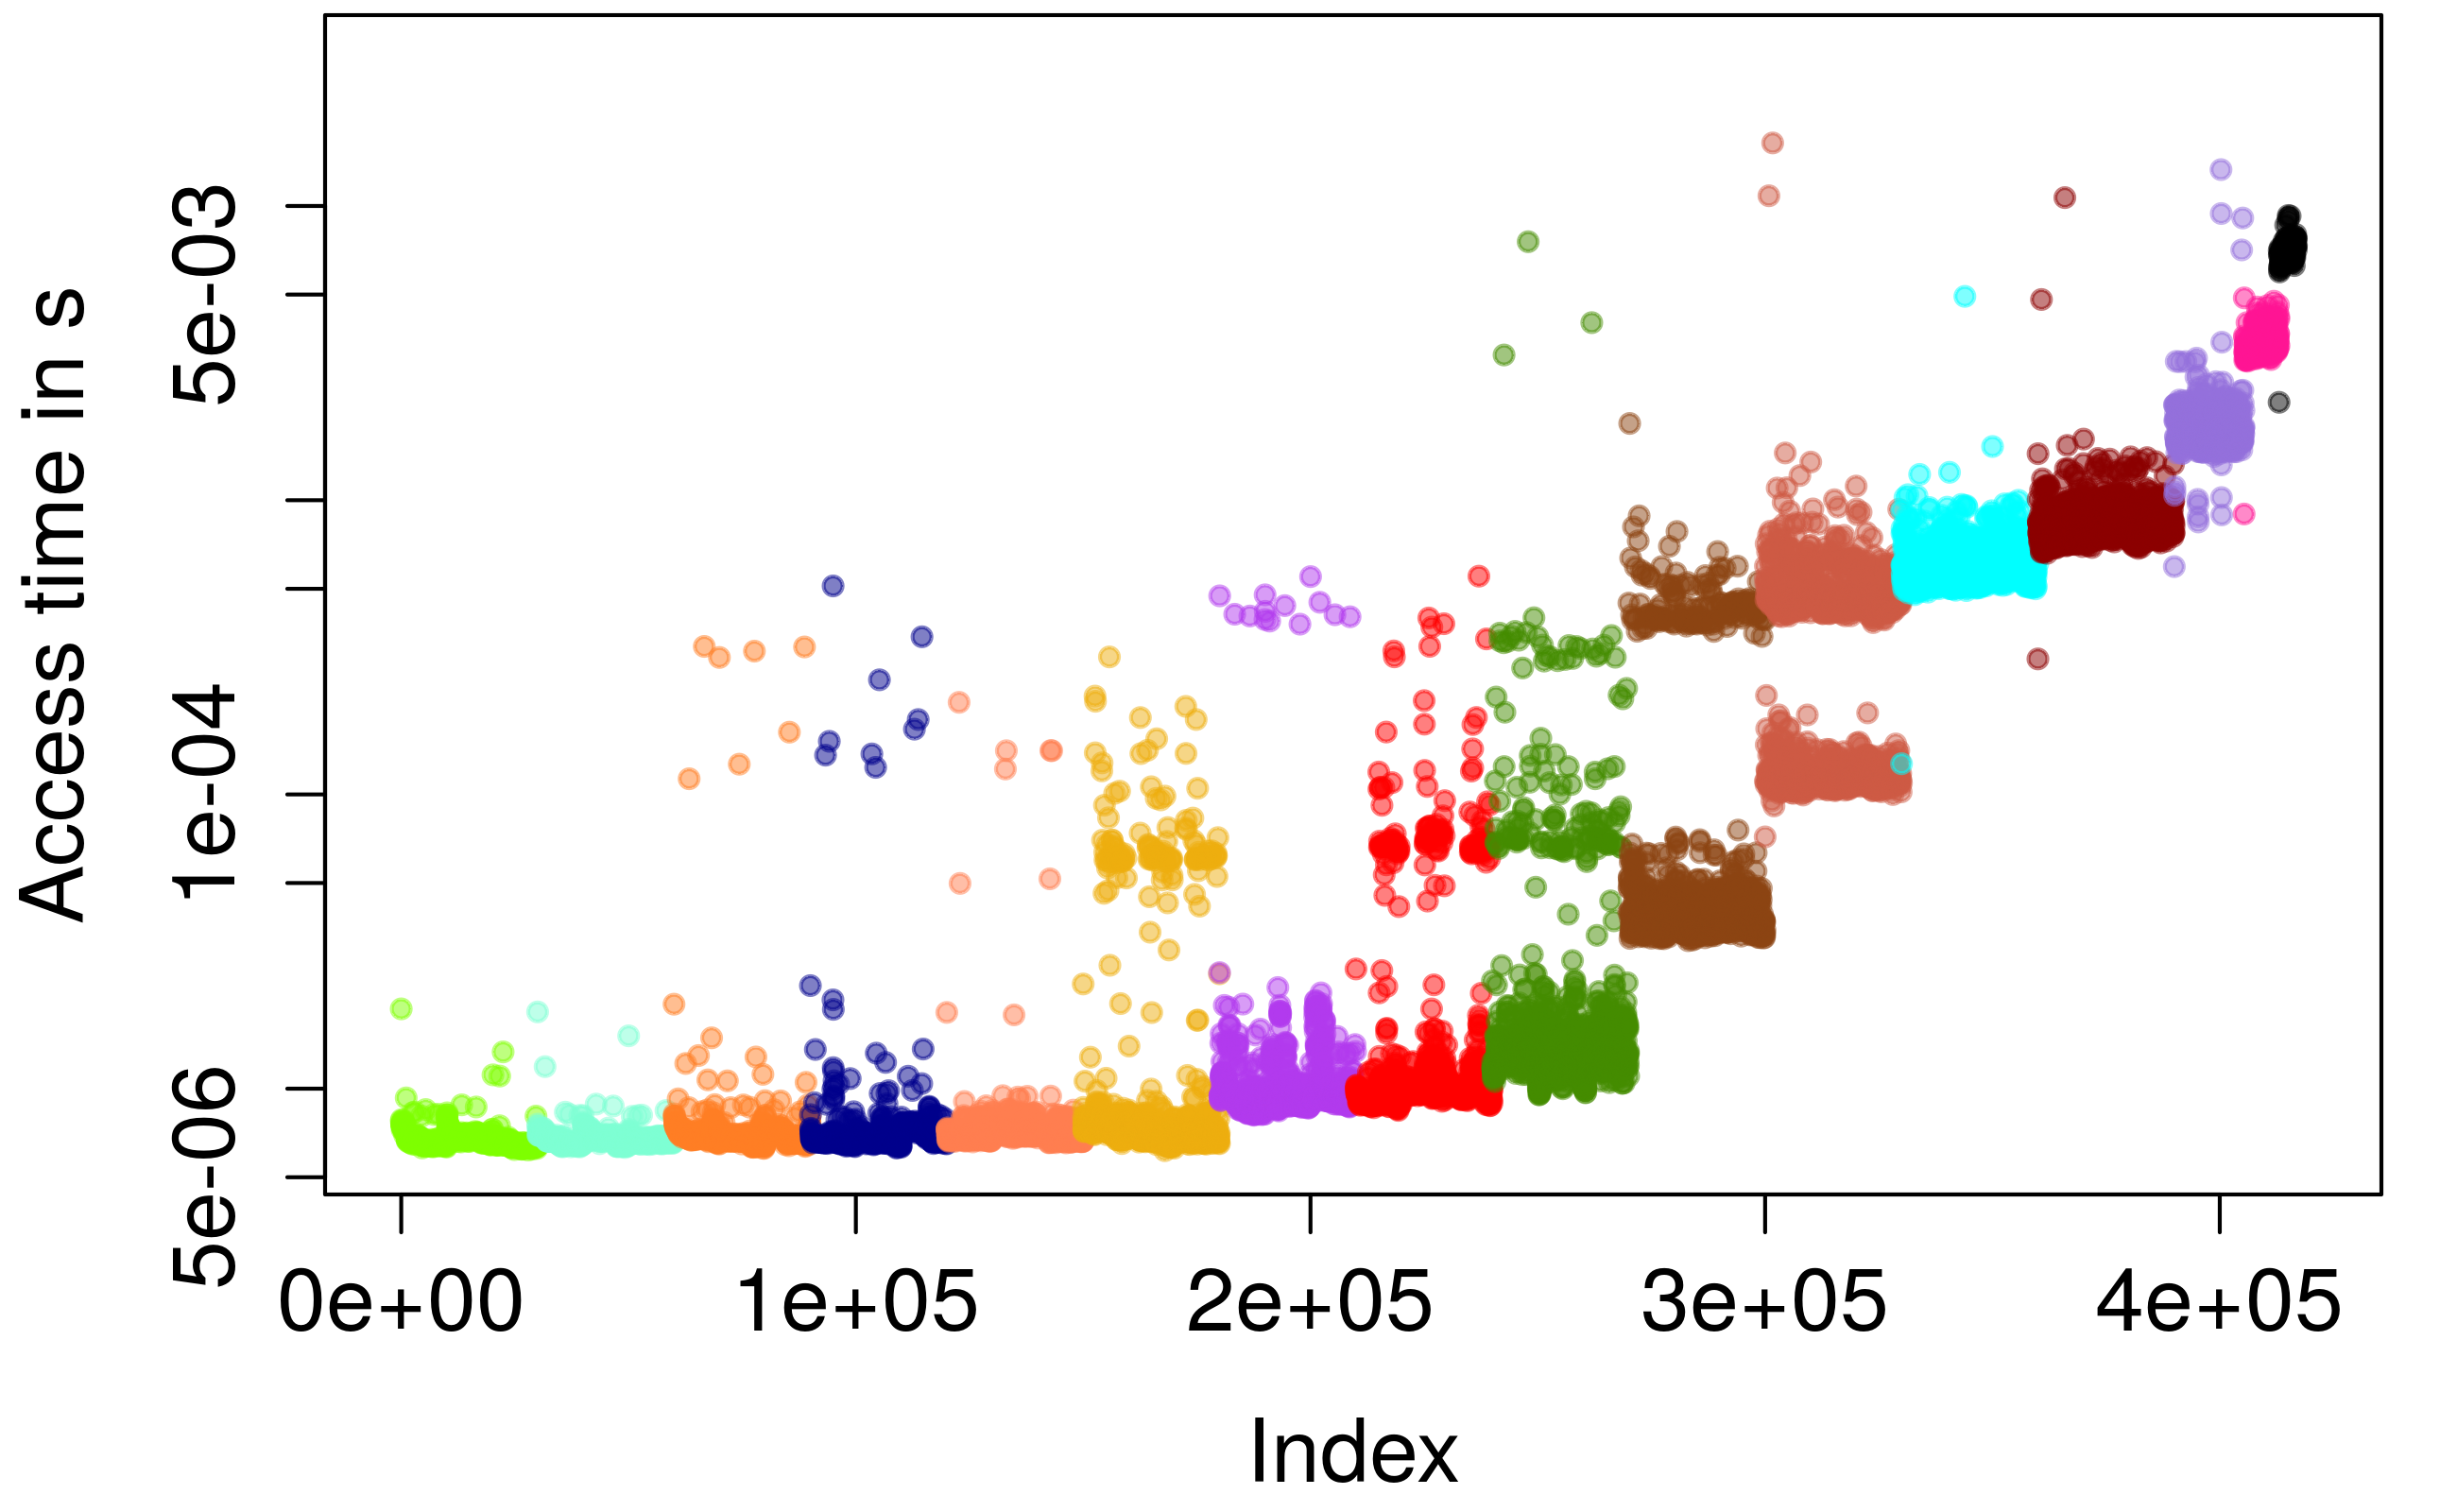
\includegraphics[width=1\linewidth]{Bilder/plot_SizeSorted_log_read_seq.png}\\
				\caption{Sequential access}
			\end{figure}
			\column{.5\textwidth}
			\begin{figure}
				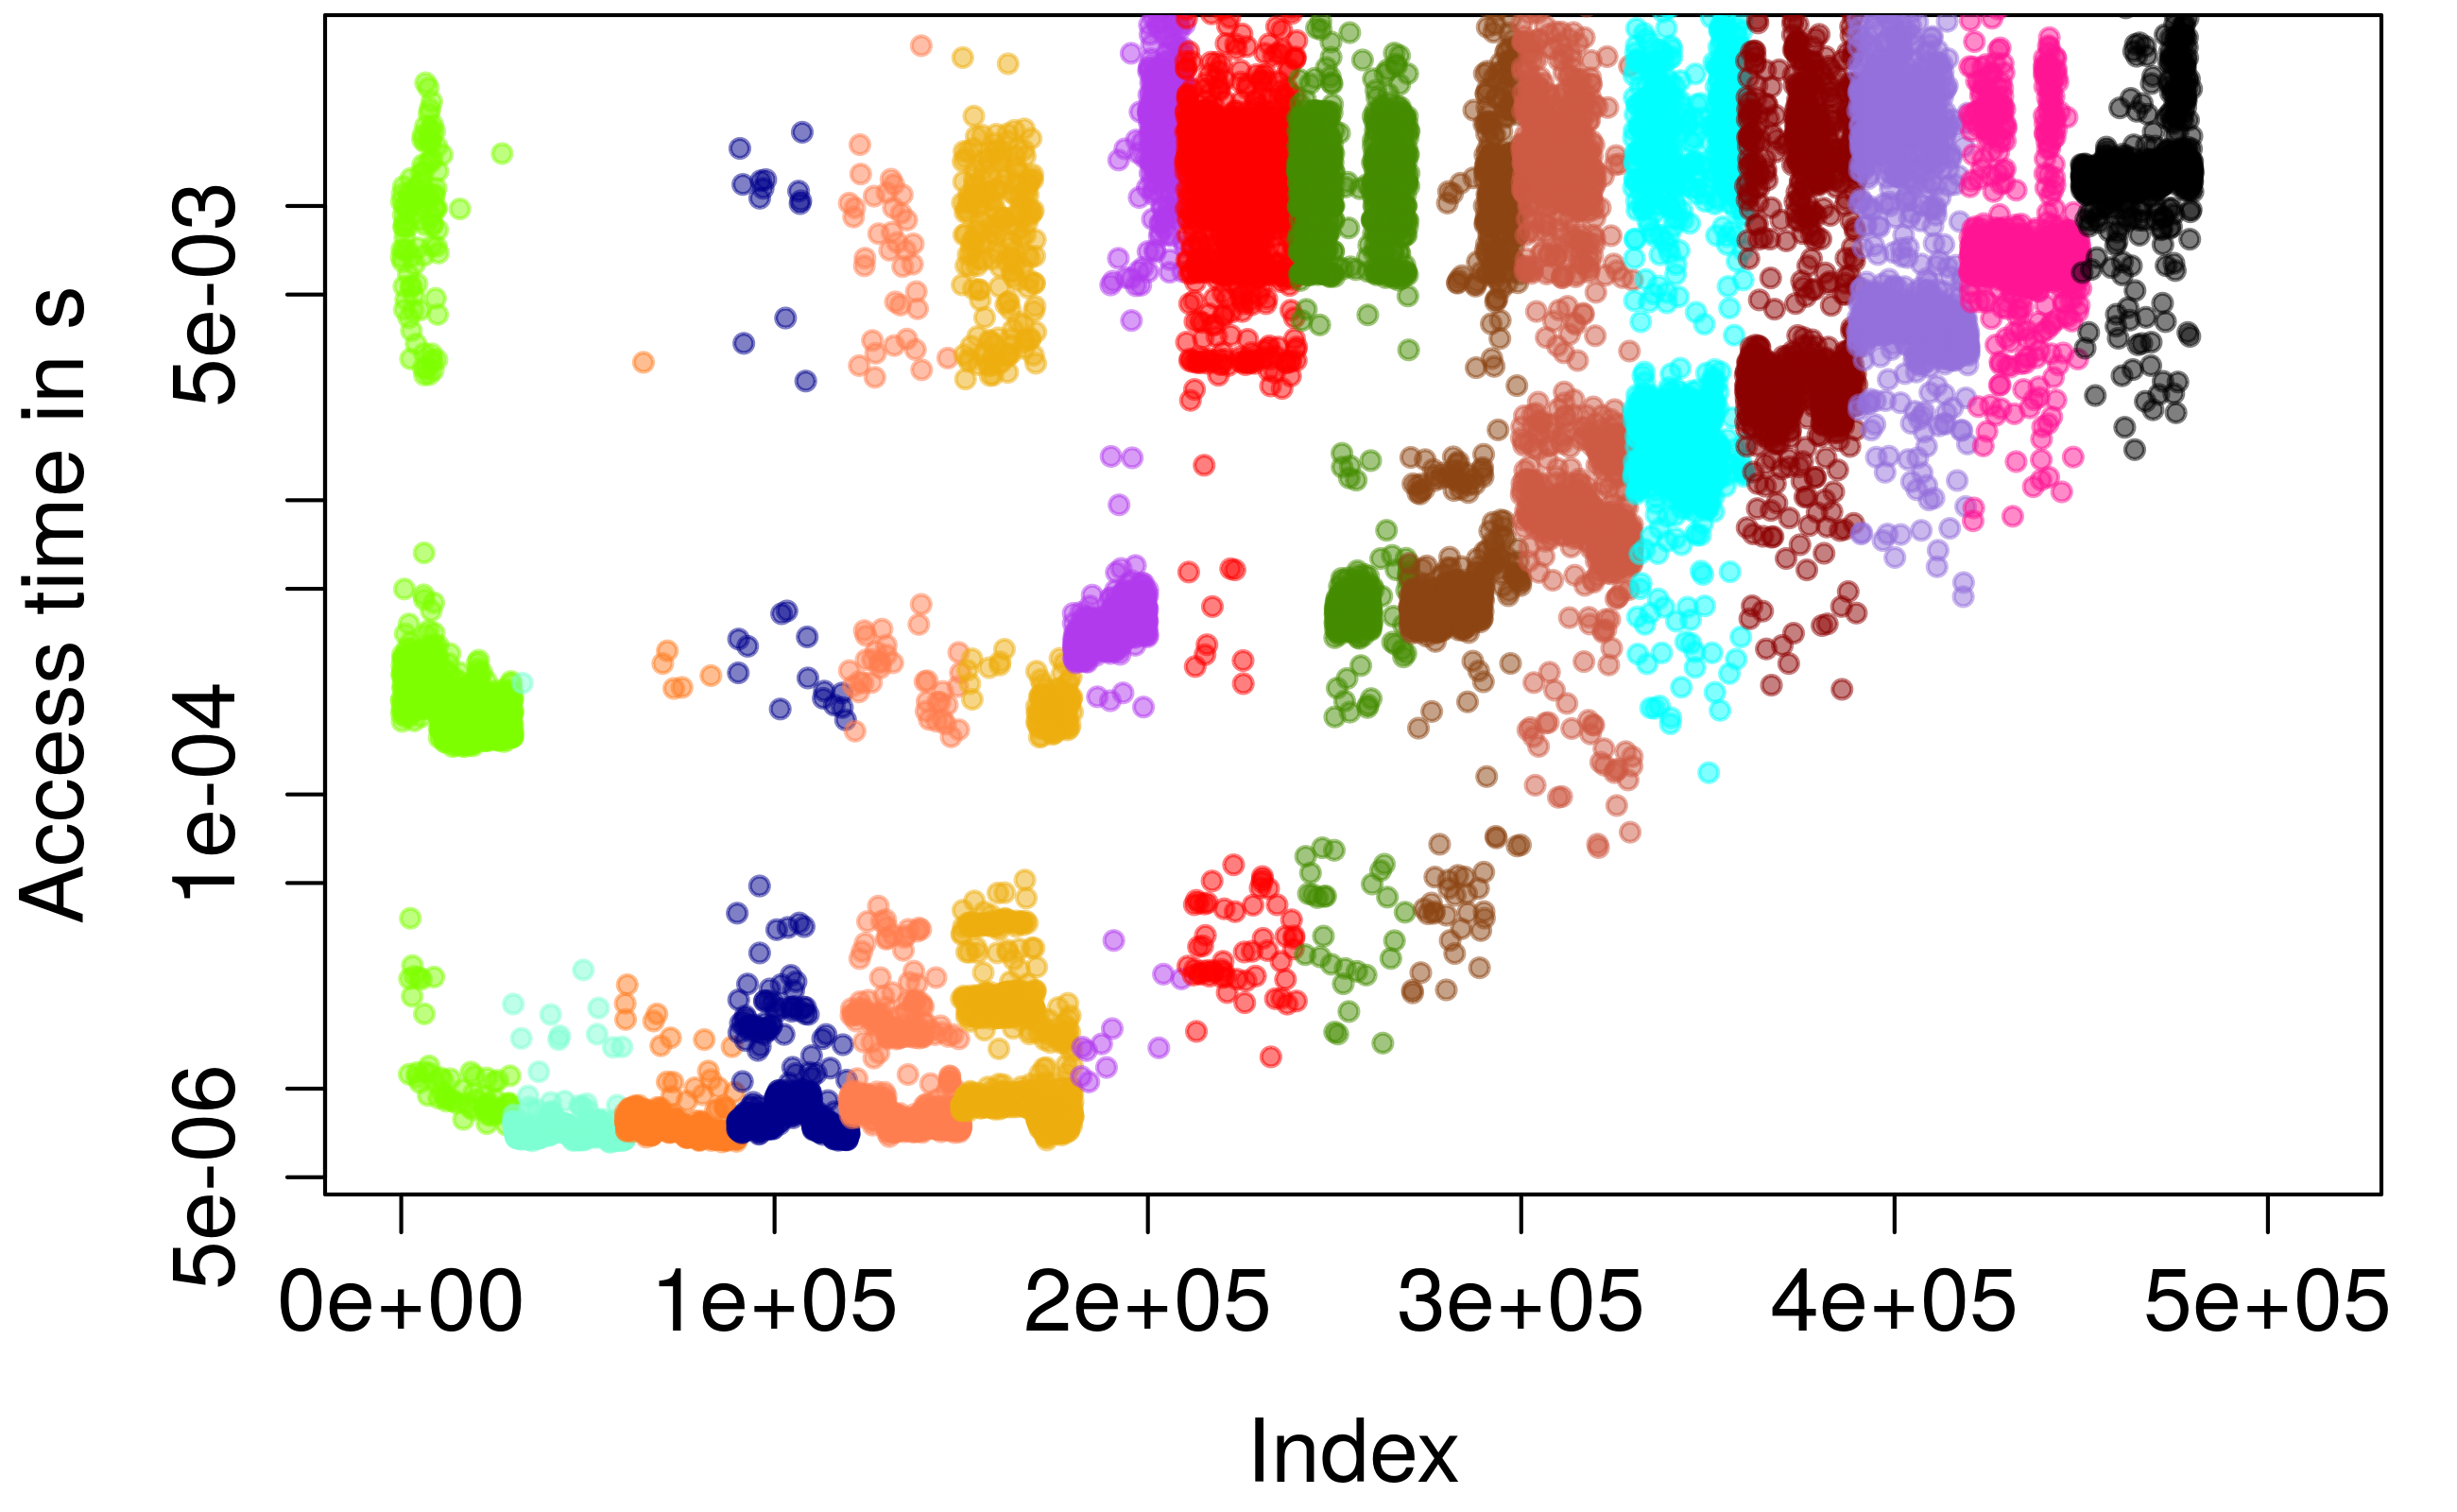
\includegraphics[width=1\linewidth]{Bilder/plot_SizeSorted_log_read_rnd.png}
				\caption{Random access}	
		\end{figure}
		\end{columns}
	\end{frame}
\end{withoutheadline}

\begin{withoutheadline}
	\begin{frame}
		\frametitle{Results}
		\begin{table}
			\footnotesize
			\vspace{0.2cm}
			\begin{tabular}{l|r|r|r|r}%
				&  \multicolumn{2}{|c}{MAE (s)}&  \multicolumn{2}{|c}{MSPE (\%)}\\ \hline
				%\toprule
				Model & seq. access & rnd. access & seq. access & rnd. access\\ \hline
				%\midrule
				Linear regression & $7.6\cdot 10^-5$ & $4.76\cdot 10^-3$ & 59 & 14185  \\
				ANN & $6.0\cdot 10^-5$ & $3.13\cdot 10^-3$ & 22 & 530 \\
				ANN + error classes & $2.0\cdot 10^-5$ & $1.03\cdot 10^-3$ & 14 & 119\\
				%\bottomrule
			\end{tabular}
		\end{table}
		\begin{figure}
			\subfloat[predictions of ANN]{
				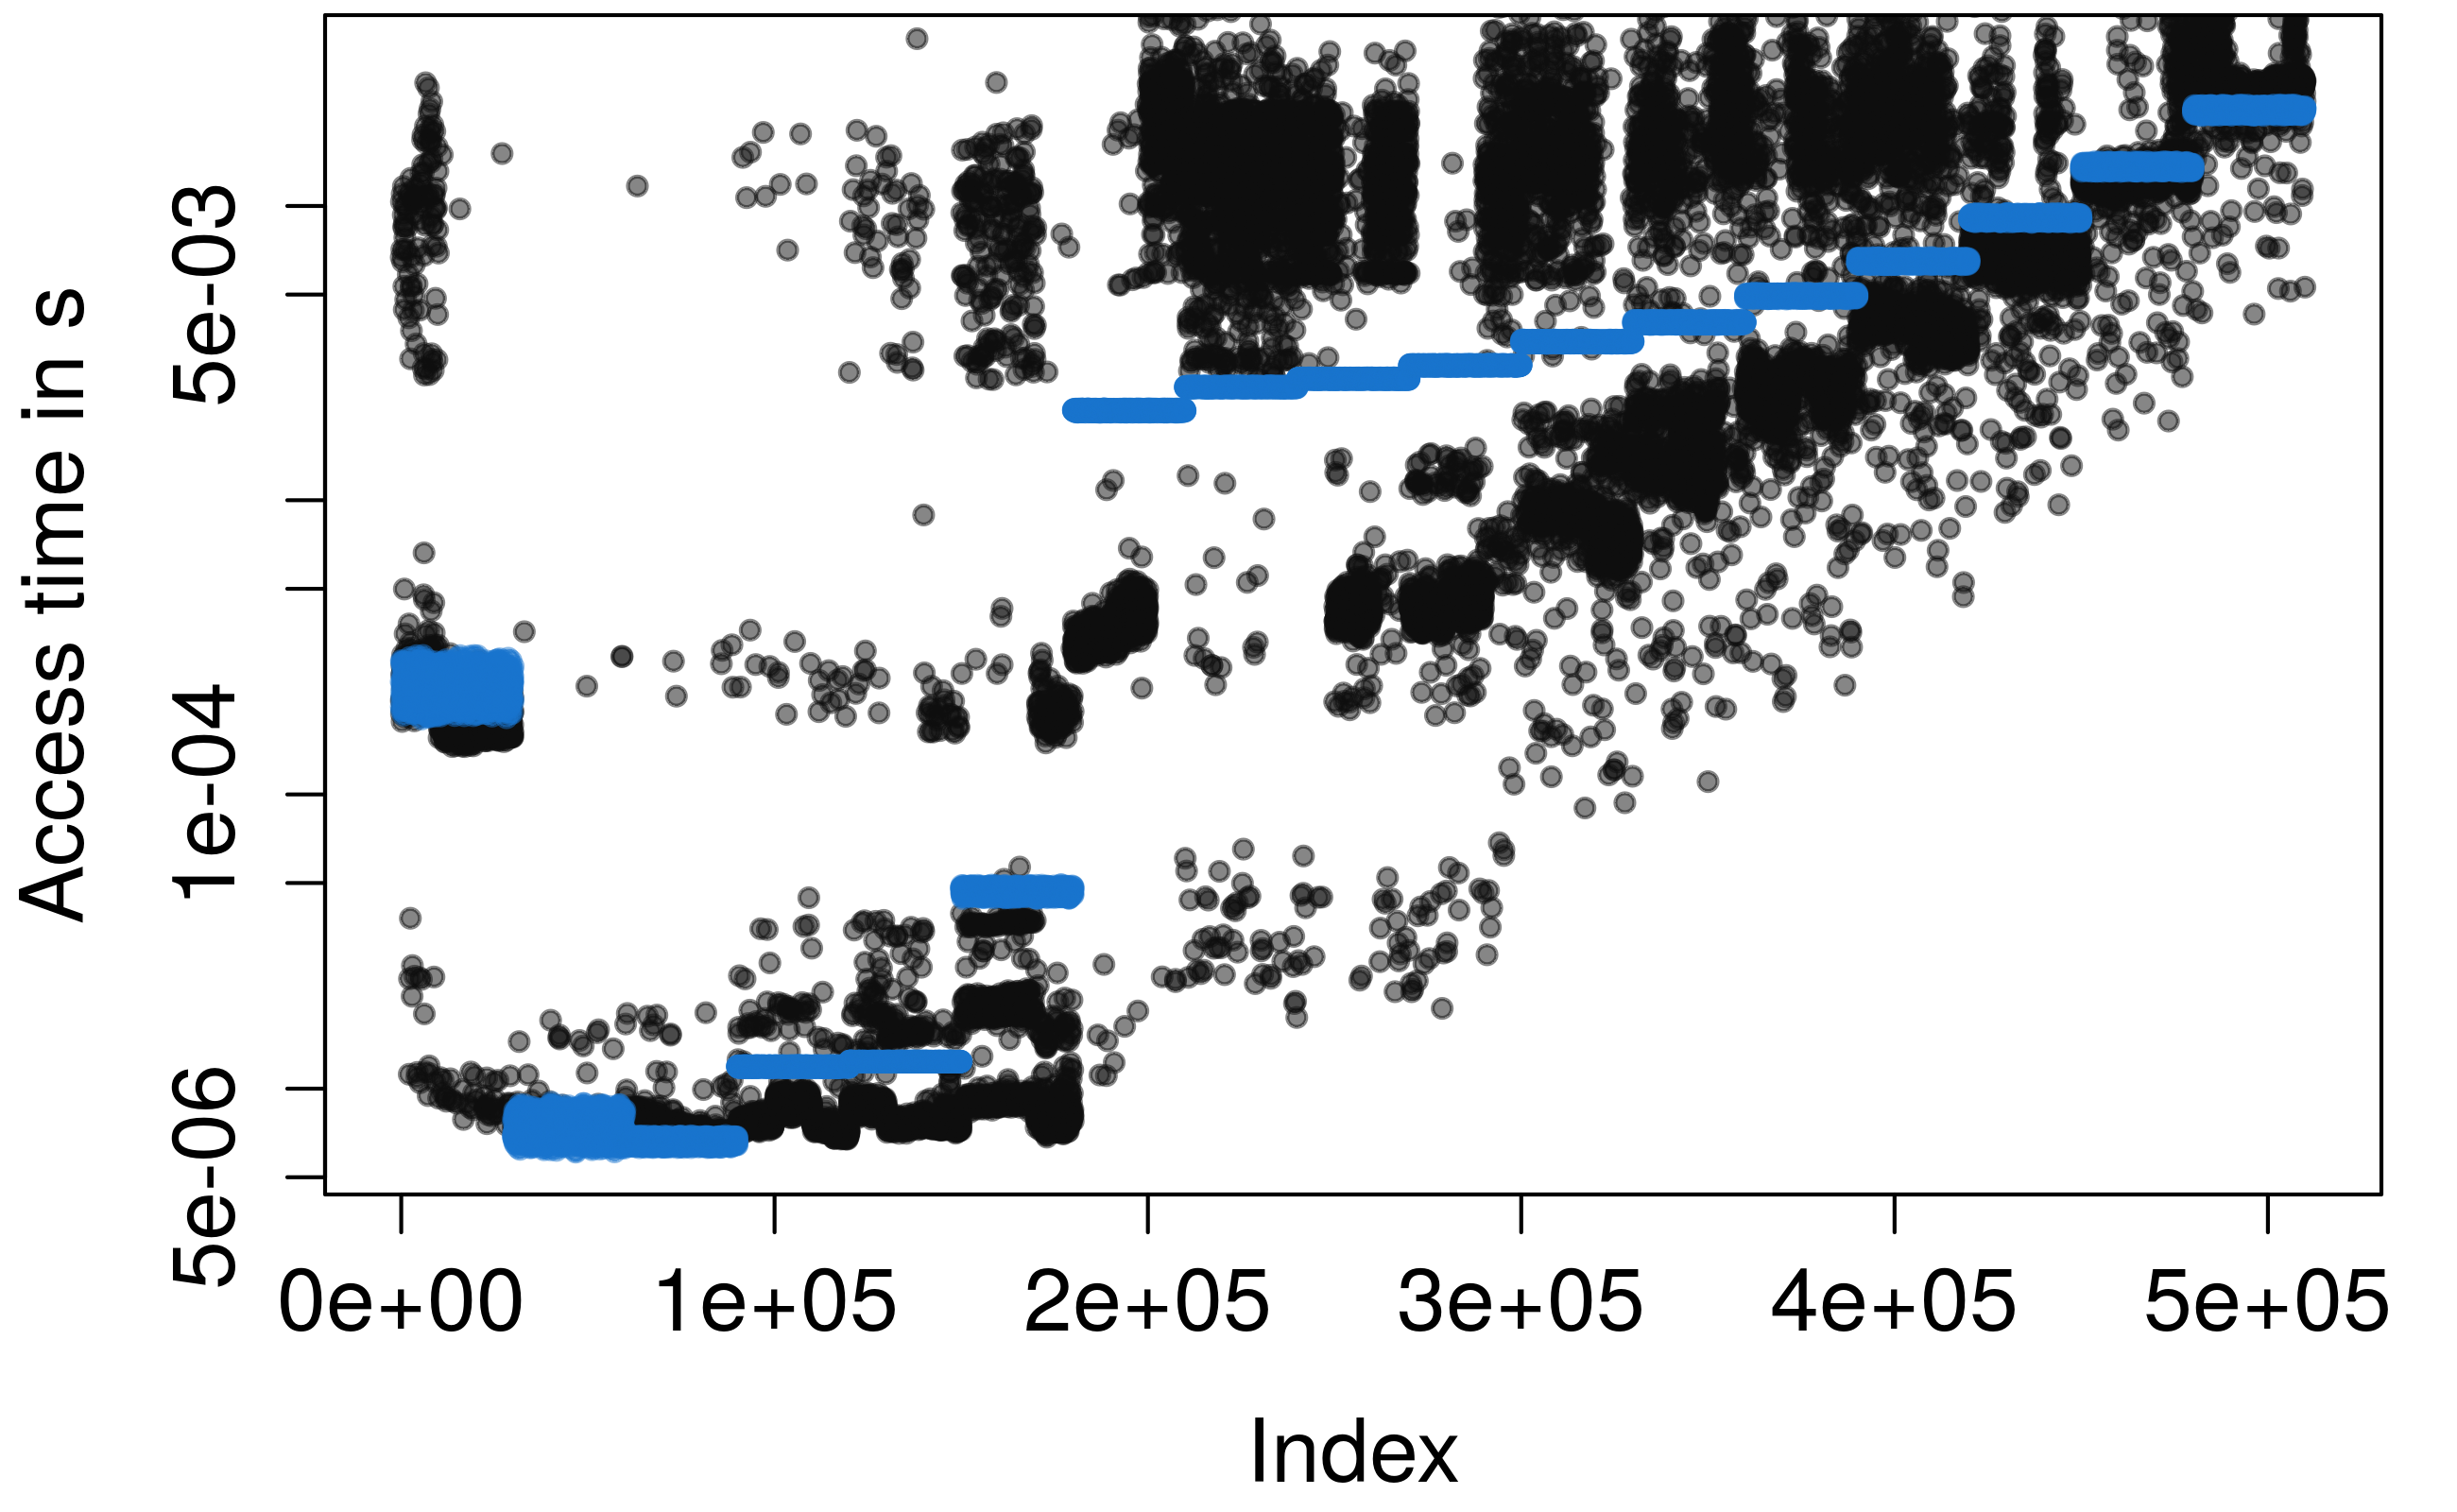
\includegraphics[width=.47\textwidth]{Bilder/plot_onlyPred_tuple1_Duration_rnd.png}
			}
			\hfill		
			\subfloat[predictions of ANN + error classes]{
				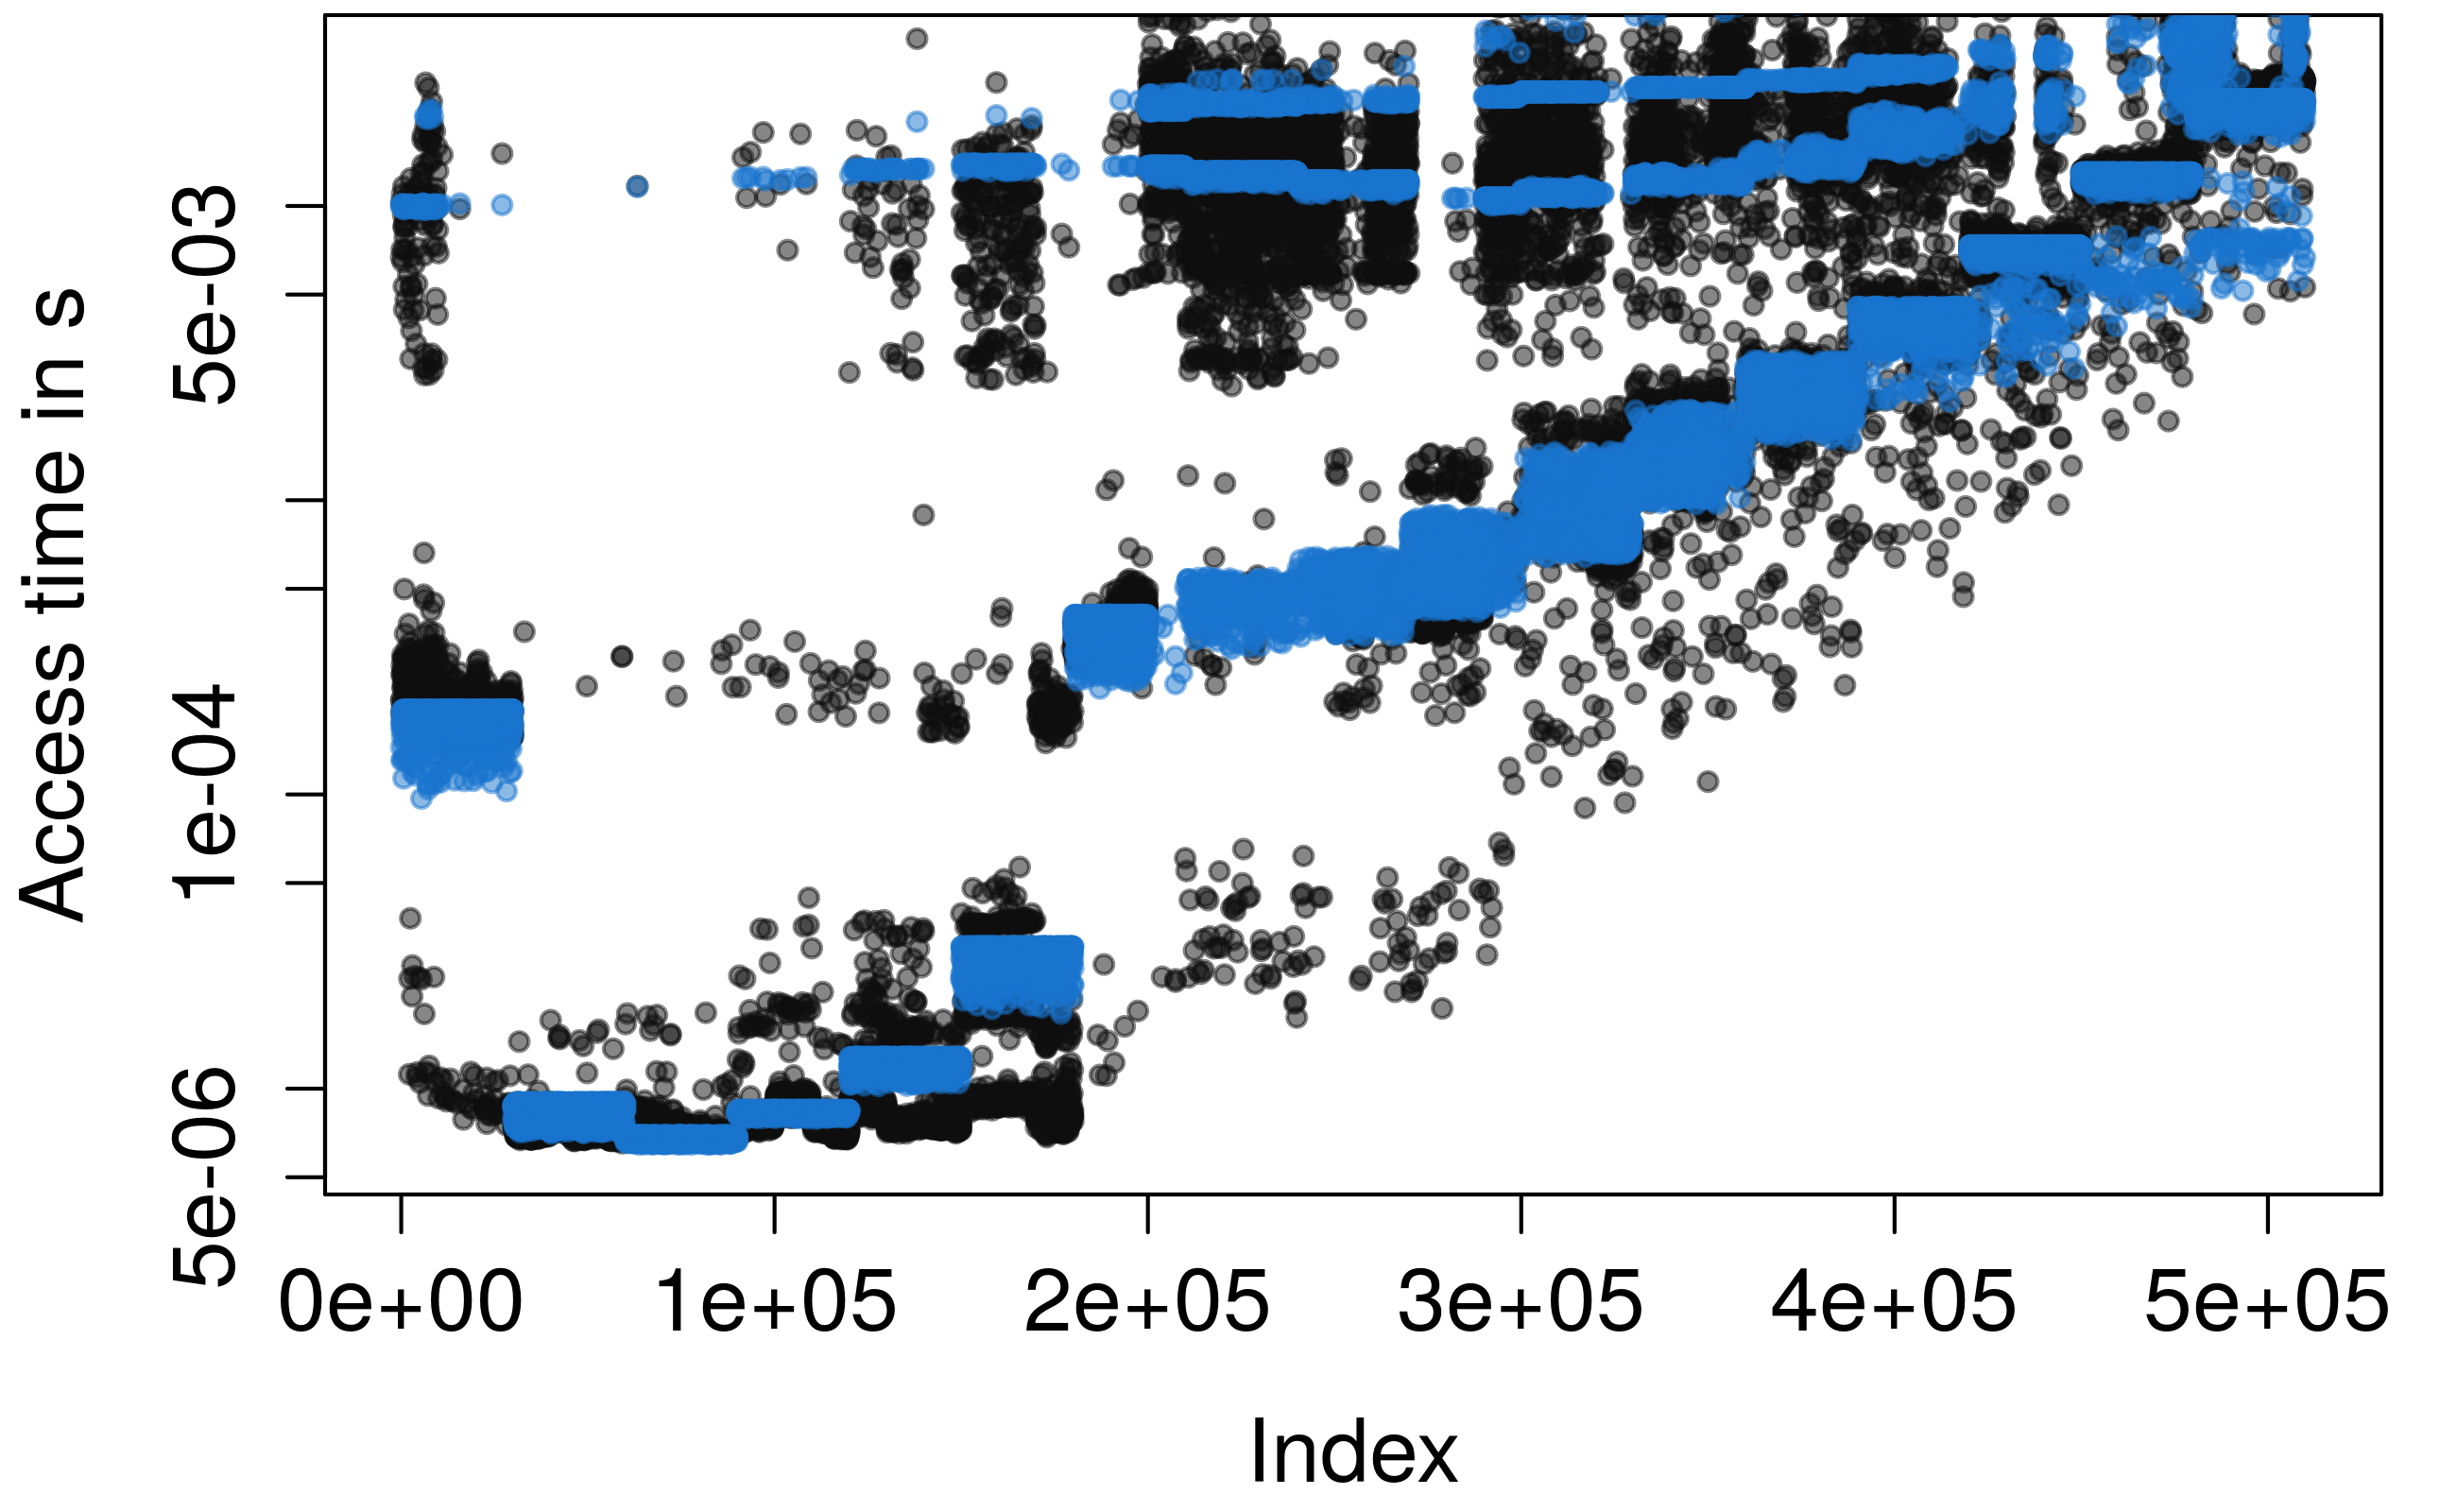
\includegraphics[width=.47\textwidth]{Bilder/plot_onlyPred_tuple1_with_error_class_from_linreg_Duration_rnd.png}
			}	
		\end{figure} 
	\end{frame}
\end{withoutheadline}

%------------------------------------------------
\begin{withoutheadline}
	\begin{frame}[plain]
		\Huge{\centerline{Thank you}}
	\end{frame}
\end{withoutheadline}

\appendix
\backupbegin
%----------------------------------------------------------------------------------------
\backupend
\end{document} 